
\section{Towards an Open Labeling Library}
\label{sec:openll}
\noindent
The fast and widespread adoption of Vulkan~\cite{vulkan} and glTF~\cite{gltf} are two recent examples of successful introductions of free and open standards.
To address industry and community needs, it is crucial not only to provide plain specifications, but to set up infrastructural means that facilitate adoption by enabling developer feedback, and providing comprehensive documentation, design guidelines and lots of examples.
Most importantly though, we consider the availability of free and open-source reference implementations as well as tools for font-asset generation and API validation to be crucial for a successful adoption of an open label library.

Though not directly intended as an extension to a specific transmission format or rendering API, the presented labeling library is designed to fit today's ecosystem of graphics rendering APIs and real-time rendering techniques.
It should provide reference implementations targeting various rendering APIs from the start.
We are currently focusing on a TypeScript-based WebGL as well as a C++-based OpenGL implementation, but are committed to subsequent ports targeting OpenGL ES and Vulkan in the future.
Both renderers are capable of laying out and rendering thousands of glyphs within a fraction of a millisecond using one of multiple rendering backends (bitmap, SDF, and spline fragments).

As of writing this paper, there is a limited number of robust font asset formats and generators available.
Our reference implementation relies on the quasi-standard bitmap font format\footnote{\url{http://www.angelcode.com/products/bmfont/}} which can be easily extended.
In order to generate font assets we used well-known font generators such as \emph{Hiero} or \emph{Littera} (deprecated due to Adobe Flash).
Due to several shortcomings, we started development of an extensible, free and open-source font-asset generator that features
\begin{itemize}
	\item interactive text rendering preview in 2D and 3D for efficient iterative font asset refinement,
	\item C++ implementation for fast texture packing, signed distance field computation and glyph rasterization~(\autoref{fig:openfag}),
	\item use via command line interface, via integration as library, or via its graphical user interface on all major platforms.
\end{itemize}

\begin{figure}[ht]
	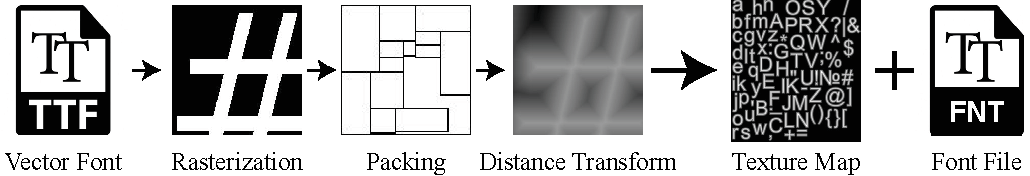
\includegraphics[width=\linewidth]{openfag}
	\vspace*{-1.5\baselineskip}
	\caption{Processing pipeline of our font asset generation library.}
	\label{fig:openfag}	
\end{figure}
